% Issue #74; owner: affan80. Input from reports/phase2/ with amsmath, graphicx
% and cite loaded. Tables are generated by scripts/prepare_dl_dataset_report.py.
% #66 evidence snapshot: 598ecb8dce4d101d118b23dd6ef6d2a1790f2615 (PR #97).
% Bibliography fragment: sections/dl_dataset.bib; consolidate in refs.bib (#80).

\section{Sequence Dataset and Regularization}
\label{sec:dl_dataset}

The sequence experiments use the FD001 run-to-failure subset of NASA
C-MAPSS~\cite{Saxena2008damage}: 100 training engines and 20,631 observed
cycles. The reference LSTM~\cite{Hochreiter1997long} has one layer of 64 units
and reads a 30-cycle sensor window. This section describes the implemented
data construction and the regularization study from issue~\#66. All reported
scores are cross-validation (CV) scores on training engines. The official
test cycles and RUL labels are not opened by the study; the frozen-model
evaluation is reserved for issue~\#71.

\subsection{Causal Windows, Stride and Padding}
For engine $i$, let $T_i$ be its final training cycle and $z_{i,t}$ its
normalized sensor vector at cycle $t$. The window ending at $t$ is
\begin{equation}
 X_{i,t}[k,:]=z_{i,\max(1,t-L+k)},\quad k=1,\ldots,L,
\end{equation}
with the first observed vector repeated on the left until the window has
exactly $L$ rows. Windows are built after sorting by engine and cycle;
they contain neither future observations nor readings from another engine.
Padding repeats the engine's own first reading, rather than zeros or the
previous engine's last reading. The label belongs to the window's final
cycle. Each PyTorch dataset item is a window--target pair; a batch has shape
$[B,L,F]$, with $F=15$ retained sensors for these folds.

Training stride $s$ counts backwards from each engine's last cycle:
$t\in\{T_i-ks:k\geq0,\ T_i-ks\geq1\}$. Thus the final cycle is always
included, and repeated-first-cycle padding gives
\begin{equation}
 N_s=\sum_i\left\lceil T_i/s\right\rceil
\end{equation}
windows. Prediction and early-stopping validation always use $s=1$,
independently of the training stride. Every cycle can therefore be predicted,
including the last cycle of an engine with fewer than $L$ observations.
At $s=1$, padding preserves the first 29 windows of every FD001 training
engine: without it, only 17,731 windows would remain, rather than 20,631.

\begin{table}[t]
\centering
\caption{Window counts for $L=30$ with left padding. Fit, ES and CV denote
fitting, inner early-stopping and outer scored engines. ES/CV use only
$s=1$; the all-training row is a reference count, not an extra study fit.}
\label{tab:dl_window_counts}
\footnotesize
\begin{tabular}{@{}lrrrr@{}}
\hline
Partition & Engines & $s=1$ & $s=2$ & $s=5$ \\
\hline
All training & 100 & 20,631 & 10,341 & 4,163 \\
Fold 1 fit & 52 & 10,588 & 5,308 & 2,134 \\
Fold 1 ES & 14 & 3,077 & -- & -- \\
Fold 1 CV & 34 & 6,966 & -- & -- \\
Fold 2 fit & 53 & 10,812 & 5,421 & 2,181 \\
Fold 2 ES & 14 & 3,167 & -- & -- \\
Fold 2 CV & 33 & 6,652 & -- & -- \\
Fold 3 fit & 53 & 10,647 & 5,336 & 2,151 \\
Fold 3 ES & 14 & 2,971 & -- & -- \\
Fold 3 CV & 33 & 7,013 & -- & -- \\
\hline
\end{tabular}

\end{table}

Table~\ref{tab:dl_window_counts} uses the same three engine-grouped folds
(split seed 42) as Phase~1. Within each outer training partition, 20\% of
its engines are held out for early stopping, again with seed 42.
Counts were checked against the actual window builder, not estimated by
dividing the number of rows by the stride. Overlapping windows are not
independent experimental units; the engine remains the unit of splitting.

\subsection{Preprocessing Within Each Fold}
The sensor list is selected from raw fitting-engine rows, before scaling.
The default variability filter removes exactly constant channels; it does
not discard a channel merely for having low variance. In all three fitting
partitions it removes $s_1,s_5,s_{10},s_{16},s_{18},s_{19}$ and retains 15
sensors, including the nearly constant $s_6$. The selected list is reused
unchanged on that fold's ES and CV engines.

The regime normalizer learns operating-setting centroids and sensor means
and population standard deviations from the fitting engines only. FD001
uses one regime. For retained sensor $j$ in regime $r$,
\begin{equation}
 z_{i,t,j}=\frac{x_{i,t,j}-\mu_{r,j}^{\mathrm{fit}}}
                         {\sigma_{r,j}^{\mathrm{fit}}}.
\end{equation}
A zero scale is replaced by one. Held-out engines use their nearest learned
regime and its saved statistics; no held-out statistics are fitted.
Engine identifier and target are metadata, and cycle index is not an input
in this reference configuration. Operating settings determine the regime
but are not direct LSTM inputs.

Fitting preprocessing before either engine split would leak held-out
distributional information. Splitting individual windows would additionally
place highly overlapping histories from the same engine on both sides.
Here the fitting, ES and outer CV engine sets are disjoint. ES loss selects
the retained training epoch~\cite{Prechelt1998early}; outer CV engines are
used only for scoring. Since model settings are selected using those CV
scores, they remain exploratory tuning results, not an unbiased final
generalization estimate.

\begin{figure*}[t]
\centering
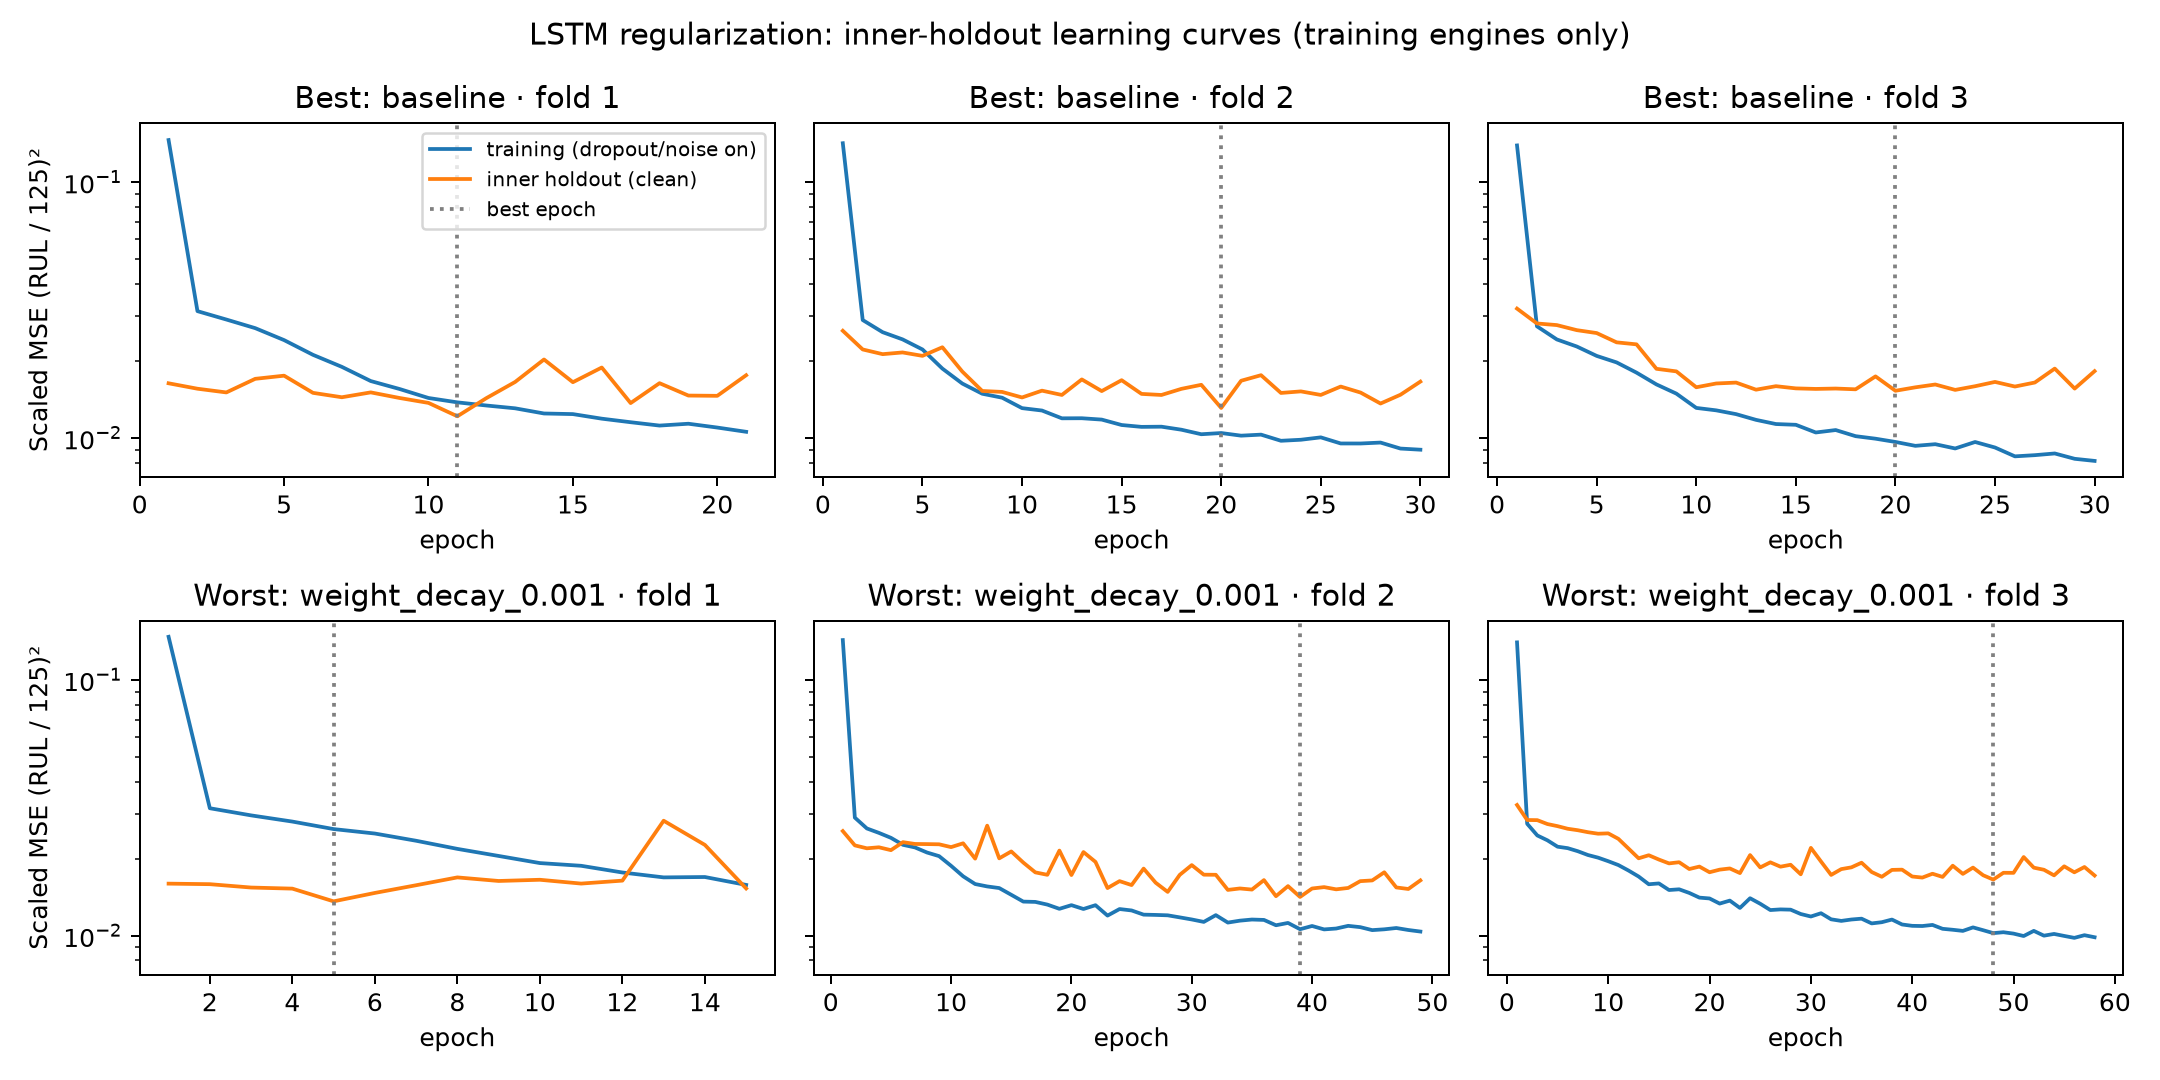
\includegraphics[width=\textwidth]{../../results/figures/fd001_regularization.png}
\caption{Learning curves from \#66 for the best capped setting (baseline)
and worst (weight decay $10^{-3}$), selected by outer CV selection RMSE.
Each column shows one fold. Training is online minibatch MSE in training
mode; the inner engine holdout is evaluated cleanly. Validation RMSE is
squared and divided by $125^2$ to match training-loss units. Vertical lines
mark retained epochs; the logarithmic axis is shared. A continuing fall in
training loss without a comparable holdout improvement is visible, but
the tested alternatives do not improve outer CV scores.}
\label{fig:dl_regularization}
\end{figure*}

\subsection{Training Target and Selection Rule}
The uncapped label is $y_{i,t}=T_i-t$. Capped training uses
$y_{i,t}^{(C)}=\min(y_{i,t},C)$, including the labels used by inner ES.
Issue~\#55 will determine the training cap and selection threshold using
training engines. Until that work lands, the study follows the existing
LSTM configuration: provisional $C=125$ and $K=130$.

For outer fold $f$, let $A_f=\{(i,t):i\text{ is scored in }f,\ y_{i,t}\leq K\}$.
The selection score is
\begin{equation}
 R_f=\sqrt{\frac{1}{|A_f|}\sum_{(i,t)\in A_f}
                  (\widehat y_{i,t}-y_{i,t})^2}.
\end{equation}
Outer scores always use true, uncapped labels. Table~\ref{tab:dl_regularization}
reports the mean of the three $R_f$ values and their sample standard
deviation, rather than a pooled cycle-level RMSE. Uncapped training is shown
beside each capped run. During optimization, targets are divided by $C$ for
capped runs, or by the largest fitting-engine label for uncapped runs;
the latter scale is independent of window stride. Predictions are converted
back to cycles before scoring.

These numerical choices are explicitly provisional. Saved out-of-fold
predictions permit rescoring when \#55 changes the selection threshold;
a changed training cap requires retraining. The official test cannot be
used to resolve either choice.

\subsection{Regularization Study and Findings}
The baseline has output dropout $p=0.3$~\cite{Srivastava2014dropout}, zero
weight decay, no input noise, stride 1 and patience 10. With one LSTM layer,
dropout acts on the final hidden state, not between recurrent layers.
Each factor is varied separately; all other baseline settings are fixed.
The shared trainer uses MSE, Adam~\cite{Kingma2015adam} at $10^{-3}$, batch
size 256, gradient clipping at norm 1, a cosine learning-rate schedule over
at most 100 epochs, CPU computation and training seed 42.

Gaussian input noise tests local perturbation robustness~\cite{Bishop1995noise}:
standard deviation is measured in fold-scaled sensor units, and new noise is
drawn for each training batch using a dedicated seeded generator. Validation
and prediction inputs remain clean, and the source arrays are unchanged.
Increasing stride reduces both windows and optimizer updates per epoch;
this is a sampling/compute comparison, not an equal-update experiment.

\begin{table}[t]
\centering
\caption{Selection RMSE (cycles), mean $\pm$ sample SD across three folds,
training seed 42. Each non-baseline row changes one factor. Capped training
uses $C=125$; both columns use true-RUL threshold $K=130$. Provisional until \#55.}
\label{tab:dl_regularization}
\footnotesize
\begin{tabular}{@{}lcc@{}}
\hline
Setting & Capped & Uncapped \\
\hline
\textbf{Baseline} & $15.78 \pm 0.44$ & $30.79 \pm 1.51$ \\
Dropout $p=0.1$ & $16.81 \pm 0.42$ & $32.43 \pm 2.05$ \\
Dropout $p=0.5$ & $16.77 \pm 1.05$ & $30.84 \pm 2.69$ \\
Weight decay $10^{-4}$ & $15.83 \pm 0.39$ & $30.97 \pm 3.21$ \\
Weight decay $10^{-3}$ & $17.60 \pm 1.00$ & $32.76 \pm 3.12$ \\
Noise $\sigma=0.01$ & $15.87 \pm 0.40$ & $30.13 \pm 1.11$ \\
Noise $\sigma=0.05$ & $16.04 \pm 0.43$ & $30.06 \pm 1.64$ \\
Stride $s=2$ & $17.47 \pm 1.03$ & $32.33 \pm 3.98$ \\
Stride $s=5$ & $17.52 \pm 0.61$ & $31.62 \pm 2.44$ \\
Patience 5 & $16.25 \pm 0.92$ & $30.79 \pm 1.51$ \\
Patience 20 & $15.78 \pm 0.44$ & $30.79 \pm 1.51$ \\
\hline
\end{tabular}

\end{table}

There are 11 settings, two target choices and three folds: 66 CPU fits,
with approximately 14.8 minutes of fitting in total. None of the tested
changes improves the baseline capped selection score of $15.78\pm0.44$.
Weight decay $10^{-4}$ ($15.83\pm0.39$) and noise 0.01 ($15.87\pm0.40$)
are close to it, rather than evidence of a gain. Patience 20 yields identical
predictions to patience 10 for both targets but takes more training.
Larger strides cost less fitting time and score worse. Noise lowers the
uncapped score slightly, but this does not change selection under the
predeclared capped-training criterion.

The recommendation is to retain dropout 0.3, weight decay 0, input noise 0,
stride 1 and patience 10; no untested combination is proposed.
Figure~\ref{fig:dl_regularization} shows the best/worst learning curves
for every fold, without averaging histories of different lengths.
The SD describes fold variation, not training-seed uncertainty or a
confidence interval. Only one training seed was tested, and the baseline
was already tuned on these folds. This null result therefore applies to
the tested settings and current provisional rule; additional seeds and
the final \#55 rule must precede any final freeze recommendation.
